\documentclass[a4paper, 11pt]{article}

\usepackage{fullpage}
\usepackage[inline]{showlabels}
\usepackage{biblatex}
\usepackage{graphicx}
\usepackage{subcaption}
\usepackage{siunitx}
\usepackage{gnuplot-lua-tikz}


\bibliography{T1.bib}

\title{Praktikum der physikalischen Chemie\\\large Versuch T1: Kalorimetrie}
\author{Janosch Ehlers (jaeh@uni-bremen.de)\\ Samed Hür (huer@uni-bremen.de)\\\small Gruppe H \\\\ \textbf{Betreuer}: Arne Wittstock (awittstock@uni-bremen.de)}
\date{25.11.2022}
\begin{document}
	\thispagestyle{empty}
	\maketitle
	\newpage

	Ziel des Versuches ist es verschiedene Physikalische Größen zu bestimmen durch die Verbrennung von Saccharose.
\section{Theoretischer Hintergrund}
	Zur Bestimmung der entstehenden Verbrennungswärme benutzt man die kalorimetrische Bombe. 
	Die Substanz wird unter Sauerstoffdruck verbrannt. 
	Mit der frei werdenden Verbrennungswärme $Q_V$ kann durch Umrechnungen die frei werdende Reaktionsenergie ($U_R$) 
	\begin{equation}
		m\cdot Q_V = n\Delta U_R
		\label{eq:UR}
	\end{equation}
	 ermittel werden.
	Die folgende Reaktionsgleichung zeigt den allgemeinen Fall der Verbrennung einer Substanz:
	\begin{equation}
	 	C_aH_bO_cN_d + \left( a + \frac{b}{4} - \frac{c}{2} \right) O_{2(g)} \rightarrow aCO_{2(g)} + \frac{b}{2} H_2O_{(1)} + \frac{d}{2} N_{2(g)} 
		\label{eq:rkt}
	\end{equation}
	 Die Molzahldifferenz kann mit 
	\begin{equation}
	 	\Delta \nu = \frac{c + d}{2} - \frac{b}{4}
		\label{eq:nu}
	\end{equation}  
	berechnet werden. 
	Der Wasserwert gibt  die Wärmekapazität des gesamten Systems wieder. 
	Die Berechnung des Wasserwertes erfolgt mit der Formel:
	\begin{equation}
		W = \frac{Q}{\Delta T}  \wedge Q = \Delta T \cdot W
		\label{eq:ww}
	\end{equation}
	Der Fehler des Wasserwertes kann über die gaußsche Fehlerfortpflanzung nach Gleichung \ref{eq:dW} oder über die Ermittlung des Mittelwertes bestimmt werden.
	\begin{equation}
		\Delta W_m = \sqrt{\left(\frac{\delta W_m}{\delta m}\cdot \Delta m\right)^2} = \frac{\Delta m \cdot Q}{\Delta T}\\	
		\label{eq:dW}
	\end{equation}
	Der Fehler von $Q$, bzw. $Q_M$ wird analog über Gleichung \ref{eq:dQ} bestimmt.
	\begin{equation}
		\Delta Q_M = \sqrt{\left( \frac{\delta Q_M}{\delta m}\cdot \Delta m \right)^2 + \left( \frac{\delta Q_M}{\delta W}\cdot \Delta W \right)^2}
     = \Delta T \cdot M \cdot \sqrt{\left( - \frac{\Delta m \cdot W}{m^2}\right)^2 + \left( \frac{\Delta W}{m}\right)^2}				
		\label{eq:dQ}
	\end{equation}

\section{Durchführung}
Zuerst wurde der Kalorimeterbecher mit ca. $2\ L$ Wasser gefüllt. 
Anschließend wurde die Benzoesäure-Tablette gewogen. 
Danach wurde die Tablette und $5\ ml$ destilliertes Wasser in die Bombe gefüllt. 
Die Temperatur wurde jede Minute gemessen. 
Nach \qty{5}{\minute} der Messung wurde die Bombe gezündet und die Messungen wurden fortgesetzt, bis die Temperatur Differenz sich nur noch minimal verändert hat. 
Diese Messung wurde zweimal durchgeführt. 
Anschließend wurden noch zwei analoge Versuche mit einem Gummibärchen (Saccharose) durchgeführt.

\section{Auswertung}
Zur Berechnung des Wasserwertes, sind die Temperaturdifferenzen über die Zeit in Abbildungen \ref{abb:benz1} und \ref{abb:Benz2} zu sehen.
Es wurde eine Lineare Regressionsgerade über die ersten 6 Werte berechnet. 
Eine Zweite wurde über die Letzen vier Werte gelegt.
Über Geogebra wurde die Fläche zwischen einer Vertikalen, den Messpunkten und den Ausgleichsgeraden berechnet.
Die Vertikale wurde so in die Abbildung gelegt, das beide Flächen gleich groß sind.
Die Schnittpunkte der Vertikalen mit den Ausgleichgeraden, gibt die Temperaturdifferenz $\Delta T_\alpha$.
Diese ist befreit von einigen Fehlern, die aus der Wärmestrahlung des Gerätes, sowie der Temperaturdifferenz zwischen Wasser und Bombe, entsteht.
In Tabelle \ref{tab:1w} sind die berechneten Ausgleichsgeraden, die Vertikalen, Probengewichte, sowie die Temperaturdifferenzen dargestellt.
Gegeben wurden uns die spezifische Verbrennungsenthalpie von Benzoesäure mit \qty{26439}{\joule\per\gram}.
Und der Verbrennungenthalpie der Baumwollfäden mit \qty{50}{\joule}.
Daraus ergibt sich nach Gleichung \ref{eq:ww} der Wasserwert.
Beispielhaft ist dies für die erste Benzoesäure-Tablette, mit \qty{0,4962}{\gram}, in Gleichung \ref{eqbsp:ww} berechnet


Dies wurde analog für die Zweite Tablette durchgeführt.
Die Temperaturdifferenzen der Proben sind in den Abbildungen \ref{abb:gummi1} und \ref{abb:gummi2} dargestellt.
Deren $\Delta T_\alpha$ kann nun wieder über Gleichung \ref{eq:ww} in eine Wärmeenergie umgerechnet werden.
Die Verbrennungswärme geteilt durch die Probenmasse gibt nun die Spezifsche Verbrennungswärme. 
Da in unserem Versuch die Druckänderung nicht Null ist, kann die Spezifische verbrennungswärme nicht ohne weiteres mit der verbrennungsenthalpie gleichgesetzt werden.
Allerdings liegen uns keine Werte über die Druckänderung vor, so definieren wir den Druck als konstant.
Die erhaltenen  Ergebnisse können aus der Tabelle \ref{tab:erg} entnommen werden.
Der Fehler der Wasserwerte ist zurückzuführen auf die Messunsicherheit, der Waage und somit nach Gleichung \ref{eq:dW} berechnet worden.
Beispielhaft ist dies für die erste Benzoesäure-Tablette in Gleichung \ref{eqbsp:dW} gezeigt.
Weiter ergiebt sich der Fehler des Spezifischen Verbrennungsenthalpie nach den Gleichungen \ref{eq:dQ} und \ref{eqbsp:dQ}.

\section{Zusatzfragen}
	\begin{enumerate}
		\item \textbf{ Was versteht man unter adiabatischer und isothermer Kalorimetrie? In welche Gruppe gehört der  vorstehende Versuch?} \\
		Bei der adiabatischen Kalorimetrie findet kein Wärmeaustausch statt und bei der isothermen Kalorimetrie bleibt die Temperatur konstant. 
		Der durchgeführte Versuch gehört zur adiabatischen Kalorimetrie.	
		\item \textbf{ Was sind atomare Bildungsenthalpien?}\\
		Atomare Bildungsenthalpien sind die Bildungsenthalpien von den einzelnen Atomen. Auch Atomisierungsenergie genannt.
		\item \textbf{ Warum muss nach der DIN-Vorschrift die Bombe vor der Verbrennung mit 5\ ml Wasser gefüllt werden? Welcher Fehler kann außerdem dadurch ausgeschlossen werden und wie groß ist er?}\\
		Die Zugabe von Wasser hilft bei der Kondensation von Wasser und verhindert das frühzeitige Stoppen der Reaktion. Wenn die Verbrennung vorzeitig abbricht, wäre der Fehler sehr groß.   
		\item  \textbf{ Wie groß ist der Fehler, wenn man bei der verbrannten Substanz näherungsweise Verbrennungsenthalpie und -energie gleichsetzt?}\\
		Wenn wir eine isobare Messung durchführen, ist der Fehler vernachlässigbar.
		$dH = dQ + pdV$
		Bei einer nicht isobaren Messung ist liegt ein großer Fehler vor.
		$dH = dQ + Vdp$
		Gehen wir in unserem Fall von einem Isobaren Prozess aus, ist der Fehler Vernachlässigbar, da $dp=0$ ist und damit der gesamt zweite Term null ist.
		In einem nicht isobaren System kann eine Abschätzung des Fehlers durch errechnen der Druckdifferenz nach dem Idealen Gasgesetz gemacht werden.
		Für die Saccharose Verbrennung liegt nach Reaktionsgleichung \ref{eq:rkt} folgende Reaktionsgleichung vor:
		$$ C_{12}H_{22}O_{11} + 12O_2 \rightarrow 12CO_2 + 11H_2O $$
		Daraus ergibt sich ein $\Delta n$ von \qty{10}{\mole}
		Das Volumen des reaktionsgefäßes ist irrelevant, da sich durch das Multiplizieren von der Druckänderung mit dem Volumen dieses herauskürzt, wenn die Druckänderung über das Ideale Gasgesetz errechnet wird.
		Weiter wird eine Temperatur von \qty{300}{\kelvin} angenommen.
		So folgt:
		\begin{align*}
			Vdp &= V\cdot\frac{\Delta nRT}{V}\\
			&= \qty{10}{\mole}\cdot\qty{8,31446}{\joule\per\mole\per\kelvin}\cdot\qty{300}{\kelvin} \\
			&= \qty{24943,38}{\joule}
		\end{align*}	
		$$ $$
	\end{enumerate}


\begin{figure}
	\centering

	\begin{subfigure}{0.4\textwidth}
		\centering
		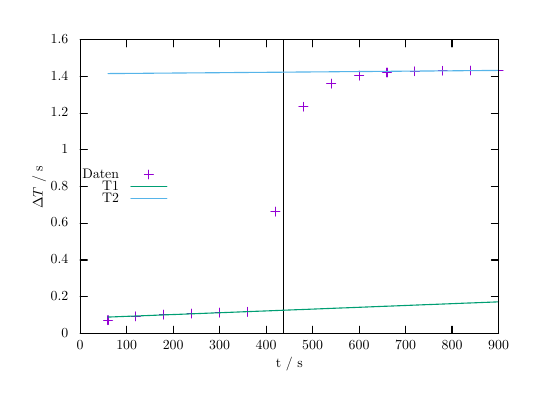
\begin{tikzpicture}[gnuplot, scale=0.5, every node/.style={scale=0.5}]
%% generated with GNUPLOT 5.4p5 (Lua 5.4; terminal rev. Jun 2020, script rev. 115)
%% Do 24 Nov 2022 22:18:53 CET
\path (0.000,0.000) rectangle (12.500,8.750);
\gpcolor{color=gp lt color border}
\gpsetlinetype{gp lt border}
\gpsetdashtype{gp dt solid}
\gpsetlinewidth{1.00}
\draw[gp path] (1.320,0.985)--(1.500,0.985);
\draw[gp path] (11.947,0.985)--(11.767,0.985);
\node[gp node right] at (1.136,0.985) {$0$};
\draw[gp path] (1.320,1.917)--(1.500,1.917);
\draw[gp path] (11.947,1.917)--(11.767,1.917);
\node[gp node right] at (1.136,1.917) {$0.2$};
\draw[gp path] (1.320,2.849)--(1.500,2.849);
\draw[gp path] (11.947,2.849)--(11.767,2.849);
\node[gp node right] at (1.136,2.849) {$0.4$};
\draw[gp path] (1.320,3.781)--(1.500,3.781);
\draw[gp path] (11.947,3.781)--(11.767,3.781);
\node[gp node right] at (1.136,3.781) {$0.6$};
\draw[gp path] (1.320,4.713)--(1.500,4.713);
\draw[gp path] (11.947,4.713)--(11.767,4.713);
\node[gp node right] at (1.136,4.713) {$0.8$};
\draw[gp path] (1.320,5.645)--(1.500,5.645);
\draw[gp path] (11.947,5.645)--(11.767,5.645);
\node[gp node right] at (1.136,5.645) {$1$};
\draw[gp path] (1.320,6.577)--(1.500,6.577);
\draw[gp path] (11.947,6.577)--(11.767,6.577);
\node[gp node right] at (1.136,6.577) {$1.2$};
\draw[gp path] (1.320,7.509)--(1.500,7.509);
\draw[gp path] (11.947,7.509)--(11.767,7.509);
\node[gp node right] at (1.136,7.509) {$1.4$};
\draw[gp path] (1.320,8.441)--(1.500,8.441);
\draw[gp path] (11.947,8.441)--(11.767,8.441);
\node[gp node right] at (1.136,8.441) {$1.6$};
\draw[gp path] (1.320,0.985)--(1.320,1.165);
\draw[gp path] (1.320,8.441)--(1.320,8.261);
\node[gp node center] at (1.320,0.677) {$0$};
\draw[gp path] (2.501,0.985)--(2.501,1.165);
\draw[gp path] (2.501,8.441)--(2.501,8.261);
\node[gp node center] at (2.501,0.677) {$100$};
\draw[gp path] (3.682,0.985)--(3.682,1.165);
\draw[gp path] (3.682,8.441)--(3.682,8.261);
\node[gp node center] at (3.682,0.677) {$200$};
\draw[gp path] (4.862,0.985)--(4.862,1.165);
\draw[gp path] (4.862,8.441)--(4.862,8.261);
\node[gp node center] at (4.862,0.677) {$300$};
\draw[gp path] (6.043,0.985)--(6.043,1.165);
\draw[gp path] (6.043,8.441)--(6.043,8.261);
\node[gp node center] at (6.043,0.677) {$400$};
\draw[gp path] (7.224,0.985)--(7.224,1.165);
\draw[gp path] (7.224,8.441)--(7.224,8.261);
\node[gp node center] at (7.224,0.677) {$500$};
\draw[gp path] (8.405,0.985)--(8.405,1.165);
\draw[gp path] (8.405,8.441)--(8.405,8.261);
\node[gp node center] at (8.405,0.677) {$600$};
\draw[gp path] (9.585,0.985)--(9.585,1.165);
\draw[gp path] (9.585,8.441)--(9.585,8.261);
\node[gp node center] at (9.585,0.677) {$700$};
\draw[gp path] (10.766,0.985)--(10.766,1.165);
\draw[gp path] (10.766,8.441)--(10.766,8.261);
\node[gp node center] at (10.766,0.677) {$800$};
\draw[gp path] (11.947,0.985)--(11.947,1.165);
\draw[gp path] (11.947,8.441)--(11.947,8.261);
\node[gp node center] at (11.947,0.677) {$900$};
\draw[gp path] (1.320,8.441)--(1.320,0.985)--(11.947,0.985)--(11.947,8.441)--cycle;
\draw[gp path](6.490,0.986)--(6.490,8.442);
\node[gp node center,rotate=-270] at (0.292,4.713) {$\Delta T$ / s};
\node[gp node center] at (6.633,0.215) {t / s};
\node[gp node right] at (2.424,5.021) {Daten};
\gpcolor{rgb color={0.580,0.000,0.827}}
\gpsetpointsize{4.00}
\gp3point{gp mark 1}{}{(2.028,1.321)}
\gp3point{gp mark 1}{}{(2.737,1.419)}
\gp3point{gp mark 1}{}{(3.445,1.461)}
\gp3point{gp mark 1}{}{(4.154,1.489)}
\gp3point{gp mark 1}{}{(4.862,1.512)}
\gp3point{gp mark 1}{}{(5.571,1.533)}
\gp3point{gp mark 1}{}{(6.279,4.078)}
\gp3point{gp mark 1}{}{(6.988,6.741)}
\gp3point{gp mark 1}{}{(7.696,7.330)}
\gp3point{gp mark 1}{}{(8.405,7.533)}
\gp3point{gp mark 1}{}{(9.113,7.611)}
\gp3point{gp mark 1}{}{(9.822,7.643)}
\gp3point{gp mark 1}{}{(10.530,7.656)}
\gp3point{gp mark 1}{}{(11.239,7.662)}
\gp3point{gp mark 1}{}{(11.947,7.660)}
\gp3point{gp mark 1}{}{(3.066,5.021)}
\gpcolor{color=gp lt color border}
\node[gp node right] at (2.424,4.713) {T1};
\gpcolor{rgb color={0.000,0.620,0.451}}
\draw[gp path] (2.608,4.713)--(3.524,4.713);
\draw[gp path] (2.028,1.399)--(2.129,1.403)--(2.229,1.407)--(2.329,1.411)--(2.429,1.415)%
  --(2.529,1.419)--(2.630,1.423)--(2.730,1.426)--(2.830,1.430)--(2.930,1.434)--(3.030,1.438)%
  --(3.131,1.442)--(3.231,1.446)--(3.331,1.450)--(3.431,1.454)--(3.531,1.458)--(3.631,1.462)%
  --(3.732,1.465)--(3.832,1.469)--(3.932,1.473)--(4.032,1.477)--(4.132,1.481)--(4.233,1.485)%
  --(4.333,1.489)--(4.433,1.493)--(4.533,1.497)--(4.633,1.501)--(4.734,1.505)--(4.834,1.508)%
  --(4.934,1.512)--(5.034,1.516)--(5.134,1.520)--(5.234,1.524)--(5.335,1.528)--(5.435,1.532)%
  --(5.535,1.536)--(5.635,1.540)--(5.735,1.544)--(5.836,1.548)--(5.936,1.551)--(6.036,1.555)%
  --(6.136,1.559)--(6.236,1.563)--(6.337,1.567)--(6.437,1.571)--(6.537,1.575)--(6.637,1.579)%
  --(6.737,1.583)--(6.837,1.587)--(6.938,1.590)--(7.038,1.594)--(7.138,1.598)--(7.238,1.602)%
  --(7.338,1.606)--(7.439,1.610)--(7.539,1.614)--(7.639,1.618)--(7.739,1.622)--(7.839,1.626)%
  --(7.940,1.630)--(8.040,1.633)--(8.140,1.637)--(8.240,1.641)--(8.340,1.645)--(8.440,1.649)%
  --(8.541,1.653)--(8.641,1.657)--(8.741,1.661)--(8.841,1.665)--(8.941,1.669)--(9.042,1.673)%
  --(9.142,1.676)--(9.242,1.680)--(9.342,1.684)--(9.442,1.688)--(9.543,1.692)--(9.643,1.696)%
  --(9.743,1.700)--(9.843,1.704)--(9.943,1.708)--(10.043,1.712)--(10.144,1.716)--(10.244,1.719)%
  --(10.344,1.723)--(10.444,1.727)--(10.544,1.731)--(10.645,1.735)--(10.745,1.739)--(10.845,1.743)%
  --(10.945,1.747)--(11.045,1.751)--(11.146,1.755)--(11.246,1.758)--(11.346,1.762)--(11.446,1.766)%
  --(11.546,1.770)--(11.646,1.774)--(11.747,1.778)--(11.847,1.782)--(11.947,1.786);
\gpcolor{color=gp lt color border}
\node[gp node right] at (2.424,4.405) {T2};
\gpcolor{rgb color={0.337,0.706,0.914}}
\draw[gp path] (2.608,4.405)--(3.524,4.405);
\draw[gp path] (2.028,7.584)--(2.129,7.585)--(2.229,7.585)--(2.329,7.586)--(2.429,7.587)%
  --(2.529,7.588)--(2.630,7.589)--(2.730,7.589)--(2.830,7.590)--(2.930,7.591)--(3.030,7.592)%
  --(3.131,7.593)--(3.231,7.594)--(3.331,7.594)--(3.431,7.595)--(3.531,7.596)--(3.631,7.597)%
  --(3.732,7.598)--(3.832,7.598)--(3.932,7.599)--(4.032,7.600)--(4.132,7.601)--(4.233,7.602)%
  --(4.333,7.602)--(4.433,7.603)--(4.533,7.604)--(4.633,7.605)--(4.734,7.606)--(4.834,7.606)%
  --(4.934,7.607)--(5.034,7.608)--(5.134,7.609)--(5.234,7.610)--(5.335,7.611)--(5.435,7.611)%
  --(5.535,7.612)--(5.635,7.613)--(5.735,7.614)--(5.836,7.615)--(5.936,7.615)--(6.036,7.616)%
  --(6.136,7.617)--(6.236,7.618)--(6.337,7.619)--(6.437,7.619)--(6.537,7.620)--(6.637,7.621)%
  --(6.737,7.622)--(6.837,7.623)--(6.938,7.624)--(7.038,7.624)--(7.138,7.625)--(7.238,7.626)%
  --(7.338,7.627)--(7.439,7.628)--(7.539,7.628)--(7.639,7.629)--(7.739,7.630)--(7.839,7.631)%
  --(7.940,7.632)--(8.040,7.632)--(8.140,7.633)--(8.240,7.634)--(8.340,7.635)--(8.440,7.636)%
  --(8.541,7.636)--(8.641,7.637)--(8.741,7.638)--(8.841,7.639)--(8.941,7.640)--(9.042,7.641)%
  --(9.142,7.641)--(9.242,7.642)--(9.342,7.643)--(9.442,7.644)--(9.543,7.645)--(9.643,7.645)%
  --(9.743,7.646)--(9.843,7.647)--(9.943,7.648)--(10.043,7.649)--(10.144,7.649)--(10.244,7.650)%
  --(10.344,7.651)--(10.444,7.652)--(10.544,7.653)--(10.645,7.654)--(10.745,7.654)--(10.845,7.655)%
  --(10.945,7.656)--(11.045,7.657)--(11.146,7.658)--(11.246,7.658)--(11.346,7.659)--(11.446,7.660)%
  --(11.546,7.661)--(11.646,7.662)--(11.747,7.662)--(11.847,7.663)--(11.947,7.664);
\gpcolor{color=gp lt color border}
\draw[gp path] (1.320,8.441)--(1.320,0.985)--(11.947,0.985)--(11.947,8.441)--cycle;
%% coordinates of the plot area
\gpdefrectangularnode{gp plot 1}{\pgfpoint{1.320cm}{0.985cm}}{\pgfpoint{11.947cm}{8.441cm}}
\end{tikzpicture}
%% gnuplot variables

		\caption{Temperaturdifferenzen der er}
	\end{subfigure}
	\hspace{5mm}
	\begin{subfigure}{0.4\textwidth}
		\centering
		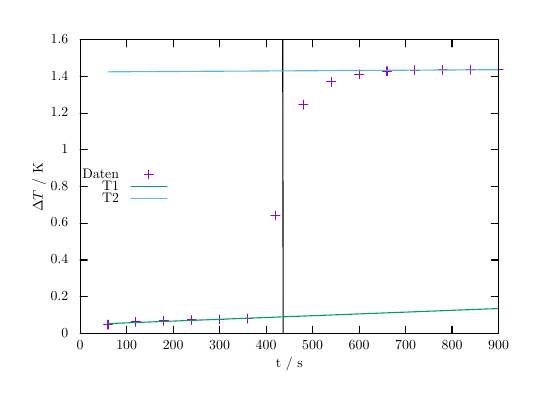
\begin{tikzpicture}[gnuplot, scale=0.5, every node/.style={scale=0.5}]
%% generated with GNUPLOT 5.4p5 (Lua 5.4; terminal rev. Jun 2020, script rev. 115)
%% Do 24 Nov 2022 22:18:53 CET
\path (0.000,0.000) rectangle (12.500,8.750);
\gpcolor{color=gp lt color border}
\gpsetlinetype{gp lt border}
\gpsetdashtype{gp dt solid}
\gpsetlinewidth{1.00}
\draw[gp path] (1.320,0.985)--(1.500,0.985);
\draw[gp path] (11.947,0.985)--(11.767,0.985);
\node[gp node right] at (1.136,0.985) {$0$};
\draw[gp path] (1.320,1.917)--(1.500,1.917);
\draw[gp path] (11.947,1.917)--(11.767,1.917);
\node[gp node right] at (1.136,1.917) {$0.2$};
\draw[gp path] (1.320,2.849)--(1.500,2.849);
\draw[gp path] (11.947,2.849)--(11.767,2.849);
\node[gp node right] at (1.136,2.849) {$0.4$};
\draw[gp path] (1.320,3.781)--(1.500,3.781);
\draw[gp path] (11.947,3.781)--(11.767,3.781);
\node[gp node right] at (1.136,3.781) {$0.6$};
\draw[gp path] (1.320,4.713)--(1.500,4.713);
\draw[gp path] (11.947,4.713)--(11.767,4.713);
\node[gp node right] at (1.136,4.713) {$0.8$};
\draw[gp path] (1.320,5.645)--(1.500,5.645);
\draw[gp path] (11.947,5.645)--(11.767,5.645);
\node[gp node right] at (1.136,5.645) {$1$};
\draw[gp path] (1.320,6.577)--(1.500,6.577);
\draw[gp path] (11.947,6.577)--(11.767,6.577);
\node[gp node right] at (1.136,6.577) {$1.2$};
\draw[gp path] (1.320,7.509)--(1.500,7.509);
\draw[gp path] (11.947,7.509)--(11.767,7.509);
\node[gp node right] at (1.136,7.509) {$1.4$};
\draw[gp path] (1.320,8.441)--(1.500,8.441);
\draw[gp path] (11.947,8.441)--(11.767,8.441);
\node[gp node right] at (1.136,8.441) {$1.6$};
\draw[gp path] (1.320,0.985)--(1.320,1.165);
\draw[gp path] (1.320,8.441)--(1.320,8.261);
\node[gp node center] at (1.320,0.677) {$0$};
\draw[gp path] (2.501,0.985)--(2.501,1.165);
\draw[gp path] (2.501,8.441)--(2.501,8.261);
\node[gp node center] at (2.501,0.677) {$100$};
\draw[gp path] (3.682,0.985)--(3.682,1.165);
\draw[gp path] (3.682,8.441)--(3.682,8.261);
\node[gp node center] at (3.682,0.677) {$200$};
\draw[gp path] (4.862,0.985)--(4.862,1.165);
\draw[gp path] (4.862,8.441)--(4.862,8.261);
\node[gp node center] at (4.862,0.677) {$300$};
\draw[gp path] (6.043,0.985)--(6.043,1.165);
\draw[gp path] (6.043,8.441)--(6.043,8.261);
\node[gp node center] at (6.043,0.677) {$400$};
\draw[gp path] (7.224,0.985)--(7.224,1.165);
\draw[gp path] (7.224,8.441)--(7.224,8.261);
\node[gp node center] at (7.224,0.677) {$500$};
\draw[gp path] (8.405,0.985)--(8.405,1.165);
\draw[gp path] (8.405,8.441)--(8.405,8.261);
\node[gp node center] at (8.405,0.677) {$600$};
\draw[gp path] (9.585,0.985)--(9.585,1.165);
\draw[gp path] (9.585,8.441)--(9.585,8.261);
\node[gp node center] at (9.585,0.677) {$700$};
\draw[gp path] (10.766,0.985)--(10.766,1.165);
\draw[gp path] (10.766,8.441)--(10.766,8.261);
\node[gp node center] at (10.766,0.677) {$800$};
\draw[gp path] (11.947,0.985)--(11.947,1.165);
\draw[gp path] (11.947,8.441)--(11.947,8.261);
\node[gp node center] at (11.947,0.677) {$900$};
\draw[gp path] (1.320,8.441)--(1.320,0.985)--(11.947,0.985)--(11.947,8.441)--cycle;
\draw[gp path](6.477,0.986)--(6.465,8.442);
\node[gp node center,rotate=-270] at (0.292,4.713) {$\Delta T$ / K};
\node[gp node center] at (6.633,0.215) {t / s};
\node[gp node right] at (2.424,5.021) {Daten};
\gpcolor{rgb color={0.580,0.000,0.827}}
\gpsetpointsize{4.00}
\gp3point{gp mark 1}{}{(2.028,1.208)}
\gp3point{gp mark 1}{}{(2.737,1.278)}
\gp3point{gp mark 1}{}{(3.445,1.305)}
\gp3point{gp mark 1}{}{(4.154,1.325)}
\gp3point{gp mark 1}{}{(4.862,1.342)}
\gp3point{gp mark 1}{}{(5.571,1.358)}
\gp3point{gp mark 1}{}{(6.279,3.979)}
\gp3point{gp mark 1}{}{(6.988,6.796)}
\gp3point{gp mark 1}{}{(7.696,7.375)}
\gp3point{gp mark 1}{}{(8.405,7.567)}
\gp3point{gp mark 1}{}{(9.113,7.642)}
\gp3point{gp mark 1}{}{(9.822,7.668)}
\gp3point{gp mark 1}{}{(10.530,7.679)}
\gp3point{gp mark 1}{}{(11.239,7.682)}
\gp3point{gp mark 1}{}{(11.947,7.680)}
\gp3point{gp mark 1}{}{(3.066,5.021)}
\gpcolor{color=gp lt color border}
\node[gp node right] at (2.424,4.713) {T1};
\gpcolor{rgb color={0.000,0.620,0.451}}
\draw[gp path] (2.608,4.713)--(3.524,4.713);
\draw[gp path] (2.028,1.234)--(2.129,1.238)--(2.229,1.241)--(2.329,1.245)--(2.429,1.249)%
  --(2.529,1.253)--(2.630,1.257)--(2.730,1.261)--(2.830,1.265)--(2.930,1.268)--(3.030,1.272)%
  --(3.131,1.276)--(3.231,1.280)--(3.331,1.284)--(3.431,1.288)--(3.531,1.292)--(3.631,1.296)%
  --(3.732,1.299)--(3.832,1.303)--(3.932,1.307)--(4.032,1.311)--(4.132,1.315)--(4.233,1.319)%
  --(4.333,1.323)--(4.433,1.326)--(4.533,1.330)--(4.633,1.334)--(4.734,1.338)--(4.834,1.342)%
  --(4.934,1.346)--(5.034,1.350)--(5.134,1.353)--(5.234,1.357)--(5.335,1.361)--(5.435,1.365)%
  --(5.535,1.369)--(5.635,1.373)--(5.735,1.377)--(5.836,1.381)--(5.936,1.384)--(6.036,1.388)%
  --(6.136,1.392)--(6.236,1.396)--(6.337,1.400)--(6.437,1.404)--(6.537,1.408)--(6.637,1.411)%
  --(6.737,1.415)--(6.837,1.419)--(6.938,1.423)--(7.038,1.427)--(7.138,1.431)--(7.238,1.435)%
  --(7.338,1.438)--(7.439,1.442)--(7.539,1.446)--(7.639,1.450)--(7.739,1.454)--(7.839,1.458)%
  --(7.940,1.462)--(8.040,1.465)--(8.140,1.469)--(8.240,1.473)--(8.340,1.477)--(8.440,1.481)%
  --(8.541,1.485)--(8.641,1.489)--(8.741,1.493)--(8.841,1.496)--(8.941,1.500)--(9.042,1.504)%
  --(9.142,1.508)--(9.242,1.512)--(9.342,1.516)--(9.442,1.520)--(9.543,1.523)--(9.643,1.527)%
  --(9.743,1.531)--(9.843,1.535)--(9.943,1.539)--(10.043,1.543)--(10.144,1.547)--(10.244,1.550)%
  --(10.344,1.554)--(10.444,1.558)--(10.544,1.562)--(10.645,1.566)--(10.745,1.570)--(10.845,1.574)%
  --(10.945,1.578)--(11.045,1.581)--(11.146,1.585)--(11.246,1.589)--(11.346,1.593)--(11.446,1.597)%
  --(11.546,1.601)--(11.646,1.605)--(11.747,1.608)--(11.847,1.612)--(11.947,1.616);
\gpcolor{color=gp lt color border}
\node[gp node right] at (2.424,4.405) {T2};
\gpcolor{rgb color={0.337,0.706,0.914}}
\draw[gp path] (2.608,4.405)--(3.524,4.405);
\draw[gp path] (2.028,7.628)--(2.129,7.629)--(2.229,7.630)--(2.329,7.630)--(2.429,7.631)%
  --(2.529,7.631)--(2.630,7.632)--(2.730,7.632)--(2.830,7.633)--(2.930,7.633)--(3.030,7.634)%
  --(3.131,7.634)--(3.231,7.635)--(3.331,7.636)--(3.431,7.636)--(3.531,7.637)--(3.631,7.637)%
  --(3.732,7.638)--(3.832,7.638)--(3.932,7.639)--(4.032,7.639)--(4.132,7.640)--(4.233,7.640)%
  --(4.333,7.641)--(4.433,7.642)--(4.533,7.642)--(4.633,7.643)--(4.734,7.643)--(4.834,7.644)%
  --(4.934,7.644)--(5.034,7.645)--(5.134,7.645)--(5.234,7.646)--(5.335,7.646)--(5.435,7.647)%
  --(5.535,7.648)--(5.635,7.648)--(5.735,7.649)--(5.836,7.649)--(5.936,7.650)--(6.036,7.650)%
  --(6.136,7.651)--(6.236,7.651)--(6.337,7.652)--(6.437,7.652)--(6.537,7.653)--(6.637,7.654)%
  --(6.737,7.654)--(6.837,7.655)--(6.938,7.655)--(7.038,7.656)--(7.138,7.656)--(7.238,7.657)%
  --(7.338,7.657)--(7.439,7.658)--(7.539,7.658)--(7.639,7.659)--(7.739,7.660)--(7.839,7.660)%
  --(7.940,7.661)--(8.040,7.661)--(8.140,7.662)--(8.240,7.662)--(8.340,7.663)--(8.440,7.663)%
  --(8.541,7.664)--(8.641,7.664)--(8.741,7.665)--(8.841,7.666)--(8.941,7.666)--(9.042,7.667)%
  --(9.142,7.667)--(9.242,7.668)--(9.342,7.668)--(9.442,7.669)--(9.543,7.669)--(9.643,7.670)%
  --(9.743,7.670)--(9.843,7.671)--(9.943,7.672)--(10.043,7.672)--(10.144,7.673)--(10.244,7.673)%
  --(10.344,7.674)--(10.444,7.674)--(10.544,7.675)--(10.645,7.675)--(10.745,7.676)--(10.845,7.676)%
  --(10.945,7.677)--(11.045,7.678)--(11.146,7.678)--(11.246,7.679)--(11.346,7.679)--(11.446,7.680)%
  --(11.546,7.680)--(11.646,7.681)--(11.747,7.681)--(11.847,7.682)--(11.947,7.682);
\gpcolor{color=gp lt color border}
\draw[gp path] (1.320,8.441)--(1.320,0.985)--(11.947,0.985)--(11.947,8.441)--cycle;
%% coordinates of the plot area
\gpdefrectangularnode{gp plot 1}{\pgfpoint{1.320cm}{0.985cm}}{\pgfpoint{11.947cm}{8.441cm}}
\end{tikzpicture}
%% gnuplot variables

		\caption{fig2}
	\end{subfigure}
	\hfill
	\begin{subfigure}{0.4\textwidth}
		\centering
		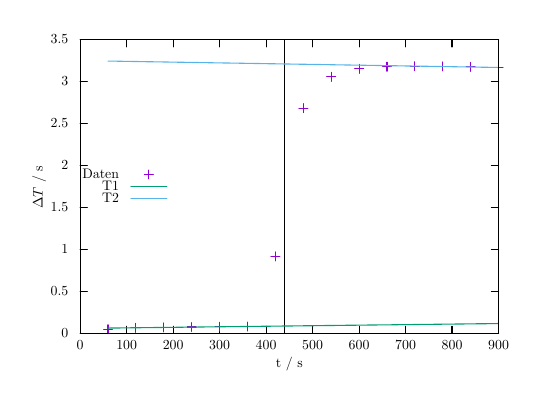
\begin{tikzpicture}[gnuplot, scale=0.5, every node/.style={scale=0.5}]
%% generated with GNUPLOT 5.4p5 (Lua 5.4; terminal rev. Jun 2020, script rev. 115)
%% Do 24 Nov 2022 22:18:53 CET
\path (0.000,0.000) rectangle (12.500,8.750);
\gpcolor{color=gp lt color border}
\gpsetlinetype{gp lt border}
\gpsetdashtype{gp dt solid}
\gpsetlinewidth{1.00}
\draw[gp path] (1.320,0.985)--(1.500,0.985);
\draw[gp path] (11.947,0.985)--(11.767,0.985);
\node[gp node right] at (1.136,0.985) {$0$};
\draw[gp path] (1.320,2.050)--(1.500,2.050);
\draw[gp path] (11.947,2.050)--(11.767,2.050);
\node[gp node right] at (1.136,2.050) {$0.5$};
\draw[gp path] (1.320,3.115)--(1.500,3.115);
\draw[gp path] (11.947,3.115)--(11.767,3.115);
\node[gp node right] at (1.136,3.115) {$1$};
\draw[gp path] (1.320,4.180)--(1.500,4.180);
\draw[gp path] (11.947,4.180)--(11.767,4.180);
\node[gp node right] at (1.136,4.180) {$1.5$};
\draw[gp path] (1.320,5.246)--(1.500,5.246);
\draw[gp path] (11.947,5.246)--(11.767,5.246);
\node[gp node right] at (1.136,5.246) {$2$};
\draw[gp path] (1.320,6.311)--(1.500,6.311);
\draw[gp path] (11.947,6.311)--(11.767,6.311);
\node[gp node right] at (1.136,6.311) {$2.5$};
\draw[gp path] (1.320,7.376)--(1.500,7.376);
\draw[gp path] (11.947,7.376)--(11.767,7.376);
\node[gp node right] at (1.136,7.376) {$3$};
\draw[gp path] (1.320,8.441)--(1.500,8.441);
\draw[gp path] (11.947,8.441)--(11.767,8.441);
\node[gp node right] at (1.136,8.441) {$3.5$};
\draw[gp path] (1.320,0.985)--(1.320,1.165);
\draw[gp path] (1.320,8.441)--(1.320,8.261);
\node[gp node center] at (1.320,0.677) {$0$};
\draw[gp path] (2.501,0.985)--(2.501,1.165);
\draw[gp path] (2.501,8.441)--(2.501,8.261);
\node[gp node center] at (2.501,0.677) {$100$};
\draw[gp path] (3.682,0.985)--(3.682,1.165);
\draw[gp path] (3.682,8.441)--(3.682,8.261);
\node[gp node center] at (3.682,0.677) {$200$};
\draw[gp path] (4.862,0.985)--(4.862,1.165);
\draw[gp path] (4.862,8.441)--(4.862,8.261);
\node[gp node center] at (4.862,0.677) {$300$};
\draw[gp path] (6.043,0.985)--(6.043,1.165);
\draw[gp path] (6.043,8.441)--(6.043,8.261);
\node[gp node center] at (6.043,0.677) {$400$};
\draw[gp path] (7.224,0.985)--(7.224,1.165);
\draw[gp path] (7.224,8.441)--(7.224,8.261);
\node[gp node center] at (7.224,0.677) {$500$};
\draw[gp path] (8.405,0.985)--(8.405,1.165);
\draw[gp path] (8.405,8.441)--(8.405,8.261);
\node[gp node center] at (8.405,0.677) {$600$};
\draw[gp path] (9.585,0.985)--(9.585,1.165);
\draw[gp path] (9.585,8.441)--(9.585,8.261);
\node[gp node center] at (9.585,0.677) {$700$};
\draw[gp path] (10.766,0.985)--(10.766,1.165);
\draw[gp path] (10.766,8.441)--(10.766,8.261);
\node[gp node center] at (10.766,0.677) {$800$};
\draw[gp path] (11.947,0.985)--(11.947,1.165);
\draw[gp path] (11.947,8.441)--(11.947,8.261);
\node[gp node center] at (11.947,0.677) {$900$};
\draw[gp path] (1.320,8.441)--(1.320,0.985)--(11.947,0.985)--(11.947,8.441)--cycle;
\draw[gp path](6.506,0.986)--(6.506,8.442);
\node[gp node center,rotate=-270] at (0.292,4.713) {$\Delta T$ / s};
\node[gp node center] at (6.633,0.215) {t / s};
\node[gp node right] at (2.424,5.021) {Daten};
\gpcolor{rgb color={0.580,0.000,0.827}}
\gpsetpointsize{4.00}
\gp3point{gp mark 1}{}{(2.028,1.090)}
\gp3point{gp mark 1}{}{(2.737,1.125)}
\gp3point{gp mark 1}{}{(3.445,1.138)}
\gp3point{gp mark 1}{}{(4.154,1.146)}
\gp3point{gp mark 1}{}{(4.862,1.154)}
\gp3point{gp mark 1}{}{(5.571,1.159)}
\gp3point{gp mark 1}{}{(6.279,2.941)}
\gp3point{gp mark 1}{}{(6.988,6.706)}
\gp3point{gp mark 1}{}{(7.696,7.501)}
\gp3point{gp mark 1}{}{(8.405,7.703)}
\gp3point{gp mark 1}{}{(9.113,7.758)}
\gp3point{gp mark 1}{}{(9.822,7.771)}
\gp3point{gp mark 1}{}{(10.530,7.765)}
\gp3point{gp mark 1}{}{(11.239,7.753)}
\gp3point{gp mark 1}{}{(11.947,7.737)}
\gp3point{gp mark 1}{}{(3.066,5.021)}
\gpcolor{color=gp lt color border}
\node[gp node right] at (2.424,4.713) {T1};
\gpcolor{rgb color={0.000,0.620,0.451}}
\draw[gp path] (2.608,4.713)--(3.524,4.713);
\draw[gp path] (2.028,1.120)--(2.129,1.121)--(2.229,1.122)--(2.329,1.123)--(2.429,1.124)%
  --(2.529,1.126)--(2.630,1.127)--(2.730,1.128)--(2.830,1.129)--(2.930,1.130)--(3.030,1.131)%
  --(3.131,1.132)--(3.231,1.134)--(3.331,1.135)--(3.431,1.136)--(3.531,1.137)--(3.631,1.138)%
  --(3.732,1.139)--(3.832,1.141)--(3.932,1.142)--(4.032,1.143)--(4.132,1.144)--(4.233,1.145)%
  --(4.333,1.146)--(4.433,1.148)--(4.533,1.149)--(4.633,1.150)--(4.734,1.151)--(4.834,1.152)%
  --(4.934,1.153)--(5.034,1.155)--(5.134,1.156)--(5.234,1.157)--(5.335,1.158)--(5.435,1.159)%
  --(5.535,1.160)--(5.635,1.162)--(5.735,1.163)--(5.836,1.164)--(5.936,1.165)--(6.036,1.166)%
  --(6.136,1.167)--(6.236,1.169)--(6.337,1.170)--(6.437,1.171)--(6.537,1.172)--(6.637,1.173)%
  --(6.737,1.174)--(6.837,1.176)--(6.938,1.177)--(7.038,1.178)--(7.138,1.179)--(7.238,1.180)%
  --(7.338,1.181)--(7.439,1.183)--(7.539,1.184)--(7.639,1.185)--(7.739,1.186)--(7.839,1.187)%
  --(7.940,1.188)--(8.040,1.190)--(8.140,1.191)--(8.240,1.192)--(8.340,1.193)--(8.440,1.194)%
  --(8.541,1.195)--(8.641,1.197)--(8.741,1.198)--(8.841,1.199)--(8.941,1.200)--(9.042,1.201)%
  --(9.142,1.202)--(9.242,1.203)--(9.342,1.205)--(9.442,1.206)--(9.543,1.207)--(9.643,1.208)%
  --(9.743,1.209)--(9.843,1.210)--(9.943,1.212)--(10.043,1.213)--(10.144,1.214)--(10.244,1.215)%
  --(10.344,1.216)--(10.444,1.217)--(10.544,1.219)--(10.645,1.220)--(10.745,1.221)--(10.845,1.222)%
  --(10.945,1.223)--(11.045,1.224)--(11.146,1.226)--(11.246,1.227)--(11.346,1.228)--(11.446,1.229)%
  --(11.546,1.230)--(11.646,1.231)--(11.747,1.233)--(11.847,1.234)--(11.947,1.235);
\gpcolor{color=gp lt color border}
\node[gp node right] at (2.424,4.405) {T2};
\gpcolor{rgb color={0.337,0.706,0.914}}
\draw[gp path] (2.608,4.405)--(3.524,4.405);
\draw[gp path] (2.028,7.902)--(2.129,7.900)--(2.229,7.899)--(2.329,7.897)--(2.429,7.895)%
  --(2.529,7.894)--(2.630,7.892)--(2.730,7.890)--(2.830,7.889)--(2.930,7.887)--(3.030,7.885)%
  --(3.131,7.884)--(3.231,7.882)--(3.331,7.881)--(3.431,7.879)--(3.531,7.877)--(3.631,7.876)%
  --(3.732,7.874)--(3.832,7.872)--(3.932,7.871)--(4.032,7.869)--(4.132,7.867)--(4.233,7.866)%
  --(4.333,7.864)--(4.433,7.862)--(4.533,7.861)--(4.633,7.859)--(4.734,7.857)--(4.834,7.856)%
  --(4.934,7.854)--(5.034,7.853)--(5.134,7.851)--(5.234,7.849)--(5.335,7.848)--(5.435,7.846)%
  --(5.535,7.844)--(5.635,7.843)--(5.735,7.841)--(5.836,7.839)--(5.936,7.838)--(6.036,7.836)%
  --(6.136,7.834)--(6.236,7.833)--(6.337,7.831)--(6.437,7.829)--(6.537,7.828)--(6.637,7.826)%
  --(6.737,7.825)--(6.837,7.823)--(6.938,7.821)--(7.038,7.820)--(7.138,7.818)--(7.238,7.816)%
  --(7.338,7.815)--(7.439,7.813)--(7.539,7.811)--(7.639,7.810)--(7.739,7.808)--(7.839,7.806)%
  --(7.940,7.805)--(8.040,7.803)--(8.140,7.801)--(8.240,7.800)--(8.340,7.798)--(8.440,7.797)%
  --(8.541,7.795)--(8.641,7.793)--(8.741,7.792)--(8.841,7.790)--(8.941,7.788)--(9.042,7.787)%
  --(9.142,7.785)--(9.242,7.783)--(9.342,7.782)--(9.442,7.780)--(9.543,7.778)--(9.643,7.777)%
  --(9.743,7.775)--(9.843,7.773)--(9.943,7.772)--(10.043,7.770)--(10.144,7.769)--(10.244,7.767)%
  --(10.344,7.765)--(10.444,7.764)--(10.544,7.762)--(10.645,7.760)--(10.745,7.759)--(10.845,7.757)%
  --(10.945,7.755)--(11.045,7.754)--(11.146,7.752)--(11.246,7.750)--(11.346,7.749)--(11.446,7.747)%
  --(11.546,7.745)--(11.646,7.744)--(11.747,7.742)--(11.847,7.741)--(11.947,7.739);
\gpcolor{color=gp lt color border}
\draw[gp path] (1.320,8.441)--(1.320,0.985)--(11.947,0.985)--(11.947,8.441)--cycle;
%% coordinates of the plot area
\gpdefrectangularnode{gp plot 1}{\pgfpoint{1.320cm}{0.985cm}}{\pgfpoint{11.947cm}{8.441cm}}
\end{tikzpicture}
%% gnuplot variables

		\caption{fig2}
	\end{subfigure}
	\hspace{5mm}
	\begin{subfigure}{0.4\textwidth}
		\centering
		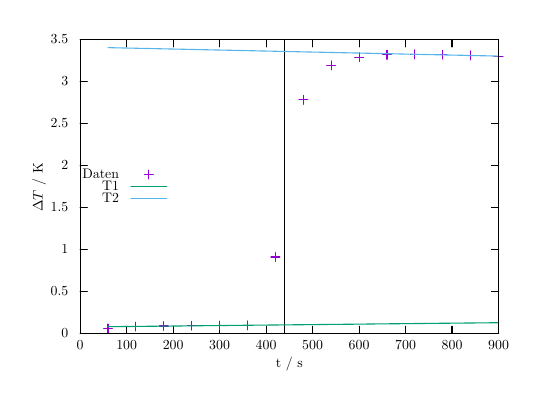
\begin{tikzpicture}[gnuplot, scale=0.5, every node/.style={scale=0.5}]
%% generated with GNUPLOT 5.4p5 (Lua 5.4; terminal rev. Jun 2020, script rev. 115)
%% Do 24 Nov 2022 22:18:53 CET
\path (0.000,0.000) rectangle (12.500,8.750);
\gpcolor{color=gp lt color border}
\gpsetlinetype{gp lt border}
\gpsetdashtype{gp dt solid}
\gpsetlinewidth{1.00}
\draw[gp path] (1.320,0.985)--(1.500,0.985);
\draw[gp path] (11.947,0.985)--(11.767,0.985);
\node[gp node right] at (1.136,0.985) {$0$};
\draw[gp path] (1.320,2.050)--(1.500,2.050);
\draw[gp path] (11.947,2.050)--(11.767,2.050);
\node[gp node right] at (1.136,2.050) {$0.5$};
\draw[gp path] (1.320,3.115)--(1.500,3.115);
\draw[gp path] (11.947,3.115)--(11.767,3.115);
\node[gp node right] at (1.136,3.115) {$1$};
\draw[gp path] (1.320,4.180)--(1.500,4.180);
\draw[gp path] (11.947,4.180)--(11.767,4.180);
\node[gp node right] at (1.136,4.180) {$1.5$};
\draw[gp path] (1.320,5.246)--(1.500,5.246);
\draw[gp path] (11.947,5.246)--(11.767,5.246);
\node[gp node right] at (1.136,5.246) {$2$};
\draw[gp path] (1.320,6.311)--(1.500,6.311);
\draw[gp path] (11.947,6.311)--(11.767,6.311);
\node[gp node right] at (1.136,6.311) {$2.5$};
\draw[gp path] (1.320,7.376)--(1.500,7.376);
\draw[gp path] (11.947,7.376)--(11.767,7.376);
\node[gp node right] at (1.136,7.376) {$3$};
\draw[gp path] (1.320,8.441)--(1.500,8.441);
\draw[gp path] (11.947,8.441)--(11.767,8.441);
\node[gp node right] at (1.136,8.441) {$3.5$};
\draw[gp path] (1.320,0.985)--(1.320,1.165);
\draw[gp path] (1.320,8.441)--(1.320,8.261);
\node[gp node center] at (1.320,0.677) {$0$};
\draw[gp path] (2.501,0.985)--(2.501,1.165);
\draw[gp path] (2.501,8.441)--(2.501,8.261);
\node[gp node center] at (2.501,0.677) {$100$};
\draw[gp path] (3.682,0.985)--(3.682,1.165);
\draw[gp path] (3.682,8.441)--(3.682,8.261);
\node[gp node center] at (3.682,0.677) {$200$};
\draw[gp path] (4.862,0.985)--(4.862,1.165);
\draw[gp path] (4.862,8.441)--(4.862,8.261);
\node[gp node center] at (4.862,0.677) {$300$};
\draw[gp path] (6.043,0.985)--(6.043,1.165);
\draw[gp path] (6.043,8.441)--(6.043,8.261);
\node[gp node center] at (6.043,0.677) {$400$};
\draw[gp path] (7.224,0.985)--(7.224,1.165);
\draw[gp path] (7.224,8.441)--(7.224,8.261);
\node[gp node center] at (7.224,0.677) {$500$};
\draw[gp path] (8.405,0.985)--(8.405,1.165);
\draw[gp path] (8.405,8.441)--(8.405,8.261);
\node[gp node center] at (8.405,0.677) {$600$};
\draw[gp path] (9.585,0.985)--(9.585,1.165);
\draw[gp path] (9.585,8.441)--(9.585,8.261);
\node[gp node center] at (9.585,0.677) {$700$};
\draw[gp path] (10.766,0.985)--(10.766,1.165);
\draw[gp path] (10.766,8.441)--(10.766,8.261);
\node[gp node center] at (10.766,0.677) {$800$};
\draw[gp path] (11.947,0.985)--(11.947,1.165);
\draw[gp path] (11.947,8.441)--(11.947,8.261);
\node[gp node center] at (11.947,0.677) {$900$};
\draw[gp path] (1.320,8.441)--(1.320,0.985)--(11.947,0.985)--(11.947,8.441)--cycle;
\draw[gp path](6.517,0.986)--(6.517,8.442);
\node[gp node center,rotate=-270] at (0.292,4.713) {$\Delta T$ / K};
\node[gp node center] at (6.633,0.215) {t / s};
\node[gp node right] at (2.424,5.021) {Daten};
\gpcolor{rgb color={0.580,0.000,0.827}}
\gpsetpointsize{4.00}
\gp3point{gp mark 1}{}{(2.028,1.108)}
\gp3point{gp mark 1}{}{(2.737,1.159)}
\gp3point{gp mark 1}{}{(3.445,1.172)}
\gp3point{gp mark 1}{}{(4.154,1.179)}
\gp3point{gp mark 1}{}{(4.862,1.184)}
\gp3point{gp mark 1}{}{(5.571,1.189)}
\gp3point{gp mark 1}{}{(6.279,2.926)}
\gp3point{gp mark 1}{}{(6.988,6.916)}
\gp3point{gp mark 1}{}{(7.696,7.791)}
\gp3point{gp mark 1}{}{(8.405,8.003)}
\gp3point{gp mark 1}{}{(9.113,8.061)}
\gp3point{gp mark 1}{}{(9.822,8.071)}
\gp3point{gp mark 1}{}{(10.530,8.062)}
\gp3point{gp mark 1}{}{(11.239,8.046)}
\gp3point{gp mark 1}{}{(11.947,8.026)}
\gp3point{gp mark 1}{}{(3.066,5.021)}
\gpcolor{color=gp lt color border}
\node[gp node right] at (2.424,4.713) {T1};
\gpcolor{rgb color={0.000,0.620,0.451}}
\draw[gp path] (2.608,4.713)--(3.524,4.713);
\draw[gp path] (2.028,1.155)--(2.129,1.156)--(2.229,1.157)--(2.329,1.158)--(2.429,1.159)%
  --(2.529,1.160)--(2.630,1.161)--(2.730,1.162)--(2.830,1.163)--(2.930,1.164)--(3.030,1.165)%
  --(3.131,1.166)--(3.231,1.167)--(3.331,1.168)--(3.431,1.169)--(3.531,1.170)--(3.631,1.171)%
  --(3.732,1.172)--(3.832,1.173)--(3.932,1.174)--(4.032,1.175)--(4.132,1.176)--(4.233,1.177)%
  --(4.333,1.179)--(4.433,1.180)--(4.533,1.181)--(4.633,1.182)--(4.734,1.183)--(4.834,1.184)%
  --(4.934,1.185)--(5.034,1.186)--(5.134,1.187)--(5.234,1.188)--(5.335,1.189)--(5.435,1.190)%
  --(5.535,1.191)--(5.635,1.192)--(5.735,1.193)--(5.836,1.194)--(5.936,1.195)--(6.036,1.196)%
  --(6.136,1.197)--(6.236,1.198)--(6.337,1.199)--(6.437,1.200)--(6.537,1.201)--(6.637,1.202)%
  --(6.737,1.203)--(6.837,1.204)--(6.938,1.205)--(7.038,1.206)--(7.138,1.207)--(7.238,1.208)%
  --(7.338,1.209)--(7.439,1.210)--(7.539,1.211)--(7.639,1.212)--(7.739,1.213)--(7.839,1.214)%
  --(7.940,1.215)--(8.040,1.216)--(8.140,1.217)--(8.240,1.218)--(8.340,1.219)--(8.440,1.220)%
  --(8.541,1.221)--(8.641,1.223)--(8.741,1.224)--(8.841,1.225)--(8.941,1.226)--(9.042,1.227)%
  --(9.142,1.228)--(9.242,1.229)--(9.342,1.230)--(9.442,1.231)--(9.543,1.232)--(9.643,1.233)%
  --(9.743,1.234)--(9.843,1.235)--(9.943,1.236)--(10.043,1.237)--(10.144,1.238)--(10.244,1.239)%
  --(10.344,1.240)--(10.444,1.241)--(10.544,1.242)--(10.645,1.243)--(10.745,1.244)--(10.845,1.245)%
  --(10.945,1.246)--(11.045,1.247)--(11.146,1.248)--(11.246,1.249)--(11.346,1.250)--(11.446,1.251)%
  --(11.546,1.252)--(11.646,1.253)--(11.747,1.254)--(11.847,1.255)--(11.947,1.256);
\gpcolor{color=gp lt color border}
\node[gp node right] at (2.424,4.405) {T2};
\gpcolor{rgb color={0.337,0.706,0.914}}
\draw[gp path] (2.608,4.405)--(3.524,4.405);
\draw[gp path] (2.028,8.243)--(2.129,8.241)--(2.229,8.238)--(2.329,8.236)--(2.429,8.234)%
  --(2.529,8.232)--(2.630,8.230)--(2.730,8.228)--(2.830,8.225)--(2.930,8.223)--(3.030,8.221)%
  --(3.131,8.219)--(3.231,8.217)--(3.331,8.215)--(3.431,8.212)--(3.531,8.210)--(3.631,8.208)%
  --(3.732,8.206)--(3.832,8.204)--(3.932,8.202)--(4.032,8.199)--(4.132,8.197)--(4.233,8.195)%
  --(4.333,8.193)--(4.433,8.191)--(4.533,8.189)--(4.633,8.186)--(4.734,8.184)--(4.834,8.182)%
  --(4.934,8.180)--(5.034,8.178)--(5.134,8.176)--(5.234,8.173)--(5.335,8.171)--(5.435,8.169)%
  --(5.535,8.167)--(5.635,8.165)--(5.735,8.163)--(5.836,8.160)--(5.936,8.158)--(6.036,8.156)%
  --(6.136,8.154)--(6.236,8.152)--(6.337,8.149)--(6.437,8.147)--(6.537,8.145)--(6.637,8.143)%
  --(6.737,8.141)--(6.837,8.139)--(6.938,8.136)--(7.038,8.134)--(7.138,8.132)--(7.238,8.130)%
  --(7.338,8.128)--(7.439,8.126)--(7.539,8.123)--(7.639,8.121)--(7.739,8.119)--(7.839,8.117)%
  --(7.940,8.115)--(8.040,8.113)--(8.140,8.110)--(8.240,8.108)--(8.340,8.106)--(8.440,8.104)%
  --(8.541,8.102)--(8.641,8.100)--(8.741,8.097)--(8.841,8.095)--(8.941,8.093)--(9.042,8.091)%
  --(9.142,8.089)--(9.242,8.087)--(9.342,8.084)--(9.442,8.082)--(9.543,8.080)--(9.643,8.078)%
  --(9.743,8.076)--(9.843,8.074)--(9.943,8.071)--(10.043,8.069)--(10.144,8.067)--(10.244,8.065)%
  --(10.344,8.063)--(10.444,8.061)--(10.544,8.058)--(10.645,8.056)--(10.745,8.054)--(10.845,8.052)%
  --(10.945,8.050)--(11.045,8.048)--(11.146,8.045)--(11.246,8.043)--(11.346,8.041)--(11.446,8.039)%
  --(11.546,8.037)--(11.646,8.035)--(11.747,8.032)--(11.847,8.030)--(11.947,8.028);
\gpcolor{color=gp lt color border}
\draw[gp path] (1.320,8.441)--(1.320,0.985)--(11.947,0.985)--(11.947,8.441)--cycle;
%% coordinates of the plot area
\gpdefrectangularnode{gp plot 1}{\pgfpoint{1.320cm}{0.985cm}}{\pgfpoint{11.947cm}{8.441cm}}
\end{tikzpicture}
%% gnuplot variables

		\caption{fig2}
	\end{subfigure}

\end{figure}


\printbibliography
\end{document}
